\Huge\documentclass{article}
\usepackage[utf8]{inputenc}

\usepackage[portuguese]{babel}
\usepackage{listings}
\usepackage{tikz}
\usepackage{booktabs}
\usepackage{float}
\usepackage{indentfirst}
\usepackage{titlesec}
\usepackage{amsmath}
\usepackage{subcaption}
\usepackage{fancybox}
\usepackage{textcomp}
\usepackage{mdframed}
\usepackage{tcolorbox}

\title{
    \Huge Computação Gráfica \\
    \vspace{1cm}
    \LARGE Trabalho Prático - Fase 1
}
\author{}
\date{}

\begin{document}

\maketitle

\begin{center}\large

\begin{tabular}{ll}
\textbf{Grupo} nr. & 38
\\\hline
a83899 & André Morais
\\
a84577 & José Pedro Silva
\\
a85954 & Luís Ribeiro
\\
a84783 & Pedro Rodrigues
\end{tabular}
\end{center}

\begin{figure}[h]
\centering

\includegraphics[height=3cm]{images/UM.png}
\end{figure}

\begin{center}
\large Mestrado Integrado em Engenharia Informática\\
        Universidade do Minho
\end{center}

\newpage

\section{Introduction}
\subsection{Contextualização}
O objetivo desta fase do projeto foi criar um gerador de vértices para quatro primitivas gráficas diferentes, sendo estas, o plano, a caixa, a esfera e o cone. Estas seriam desenhadas tendo em conta os argumentos de input do utilizador, podendo os mesmos variar entre, altura, largura, profundidade e o número de divisões.
\par Todos os vértices após serem gerados através do programa \textit{generator} são guardados num ficheiro cujo o nome é definido pelo utilizador. Após isso é adicionada uma entrada no ficheiro \textit{config.xml} com o nome do ficheiro.
\par Quando executado o programa \textit{engine}, este lê o ficheiro \textit{config.xml} e através do OpenGL desenha as imagens resultantes da união dos triângulos previamente gerados.
\newpage

\section{Arquitetura e utilização}
Nesta fase implementamos um gerador e um motor, então, os ficheiros executaveis gerados pelo nosso programa são \textit{generator} e \textit{engine}. O modo de utilização é simples, para compilar o código todo e gerar os executaveis basta correr o script \textbf{install.sh}, isto irá criar uma pasta com a \textit{build}, outra pasta com os \textit{models} e o ficheiro \textit{config.xml}.

\vspace{0.5cm}

Assim, para poder gerar qualquer figura, temos de entrar na pasta build e correr o \textbf{generator} com os argumentos necessários, isto vai fazer com que seja criado o ficheiro na pasta \textit{model} com o nome que passamos como argumento ao generator. Para conseguir ver as figuras que gerou, basta correr o engine.

\vspace{0.5cm}

Existe também um scritp \textb{uninstall} que serve para eliminar a pasta da build, os models todos criados e o ficheiro xml.

\vspace{0.5cm}

Se desejar realizar a build sem o \textit{install} então deve criar a pasta para o build e criar a pasta models.

\vspace{0.5cm}

Este programa contém também um script de demonstração que gera cada uma das figuras e depois desenha, por isso, para testar o programa e ver a demonstração, basta correr o \textit{demo.sh}.

\newpage

\section{Primitivas gráficas}

\subsection{Plane}
De modo a obter os pontos necessários para os triangulos que posteriormente formariam o plano, necessitamos apenas das dimensões do mesmo. 
Para obter o plano precisamos de quatro pontos, pois com estes conseguimos formar os quatro triângulos necessários (dois para visualizar o plano de cima e dois para visualizar o plano por baixo).

\subsection{Cálculo das coordenadas}
Uma vez que o plano se encontra centrado na origem e não possui altura, de modo a obter as coordenas, precisamos apenas de dividir as dimensões em duas partes, sendo as coordenadas genéricas dos quatro pontos:
\[A(\frac{x}{2}, 0, \frac{z}{2}) \hspace{1cm} B(\frac{x}{2}, 0, -\frac{z}{2})\]
\[C(-\frac{x}{2}, 0, -\frac{z}{2}) \hspace{1cm} D(-\frac{x}{2}, 0, \frac{z}{2})\]

\vspace{0.5cm}

\begin{figure}[h]
\centering
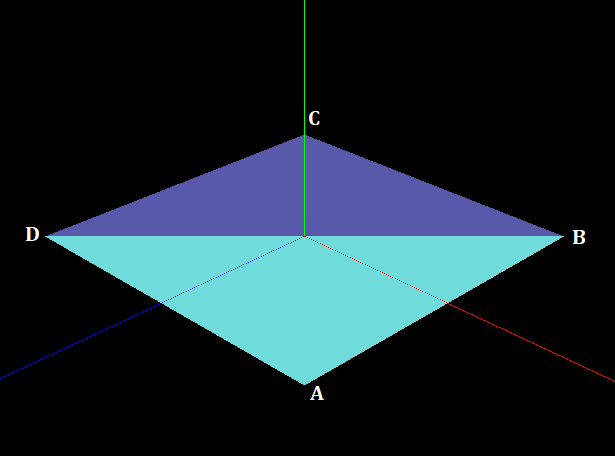
\includegraphics[width=0.7\linewidth]{images/plano.png}
\end{figure}

\subsection{Box}
Na abordagem do modelo da caixa, podemos considerar a mesma como um prima de seis faces. Numa abordagem simples e básica, cada face da caixa poderia corresponder a um plano, isto é, seriam apenas necessários dois triângulos para definir cada face. De modo a introduzir o conceito de camadas, é crucial ajustar o número de triângulos necessários para cada face.
\subsection{Cálculo das coordenadas}
Para sabermos as coordenas dos pontos que formam os triângulos, necessitamos previamente de saber o número de divisões que por sua vez fornecerá a distância entre cada ponto.
\[distanciaX = \frac{dimensaoX}{nrDivisoes + 1}\]
\[distanciaY = \frac{dimensaoY}{nrDivisoes + 1}\]
\[distanciaZ = \frac{dimensaoZ}{nrDivisoes + 1}\]
Analogamente ao plano, os vértices da caixa têm as coordenadas
\[(\frac{x}{2}, \frac{y}{2}, \frac{z}{2})\]
podendo estas ter valores negativos ou positivos. De modo a explicar o algoritmo utilizado, usemos como exemplo a face frontal da caixa e tomemos como ponto inicial o vértice do canto superior direito. Criemos então o quadrado ABCD, onde A corresponde ao ponto inicial.
\[A(\frac{x}{2}, \frac{y}{2}, \frac{z}{2})\]
\[B(\frac{x}{2} - distanciaX, \frac{y}{2}, \frac{z}{2})\]
\[C(\frac{x}{2} - distanciaX, \frac{y}{2} - distanciaY, \frac{z}{2})\]
\[D(\frac{x}{2}, \frac{y}{2} - distanciaY, \frac{z}{2})\]


Para a representação dos triângulos definidos através dos pontos acima descritos, temos que ter em conta a regra da mão direita. Representamos, então, os triângulos da seguinte maneira: ACD e ABC, para que a orientação da parte frontal esteja virada para a câmera. 
Usamos o mesmo algortimo de representação para o resto das divisões, diminuindo a coordenada \textit{x} ou \textit{y} dependendo da divisão que queremos desenhar (diminuímos \textit{y} para as divisões abaixo da inicial, e diminuímos \textit{x} para as divisões à esquerda da inicial).
O resto das faces é desenhada analogamente, variando apenas a ordem dos vértices para que estes quando formarem um triângulo sejam visíveis, isto, mais uma vez segundo a regra da mão direita. 

\subsection{Sphere}

Para o cálculo dos pontos que representam uma esfera são necessários o raio, o número de slices e o número de stacks da mesma. O número de slices corresponde ao número de camadas verticais e o número de stacks ao número de camadas horizontais da esfera, sendo assim, quanto maior forem estes números, a esfera será mais "arredondada" e precisa porque terá um número maior de pontos.

\begin{figure}[h]
\centering
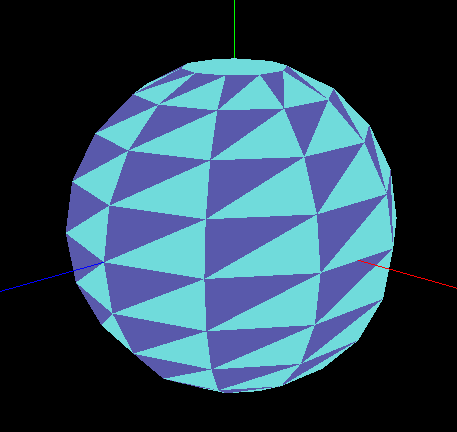
\includegraphics[width=0.7\linewidth]{images/spheredraw.png}
\end{figure}

\vspace{0.5cm}

Como podemos observar pela Figura, as camadas horizontais e verticais, formam um retângulo entre si, que por sua vez é transformado em dois triângulos. O cálculo das coordenadas dos triângulos será apresentada a seguir.

\subsubsection{Cálculo das coordenadas e das variações de $r'$}

Cada ponto tem um vetor associado a si que o liga à origem e tem norma igual ao raio, este vetor contém também dois ângulos importantes, um relativo ao eixo dos \textbf{Z ($\alpha$)} e outro relativo ao eixo dos \textbf{Y ($\beta$)}. Com estes dados passa a ser possível o cálculo das coordenadas de cada ponto utilizando regras trignométricas. Resta-nos calcular a variação do ângulo $\alpha$ e $\beta$ e do raio da circunferência menor ($r'$).

\vspace{0.5cm}

Então em cada slice, o ângulo $\alpha$ varia entre 0 e 2$\pi$ e será sempre incrementado em:
\[\frac{2\times\pi}{slices}\]

E em cada stack, o ângulo $\alpha$ varia entre $-\frac{\pi}{2}$ e $\frac{\pi}{2}$ e será sempre incrementado em:
\[\frac{\pi}{stack}\]

\vspace{0.5cm}

\begin{figure}[h]
\centering
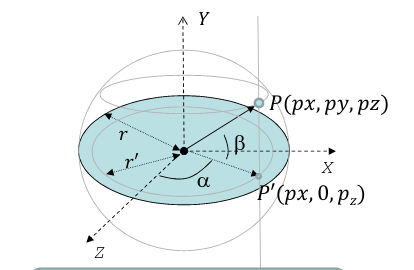
\includegraphics[width=0.7\linewidth]{images/sphere.png}
\end{figure}

Com todos estes dados e segundo as regras trignométricas, os valores das coordenadas e da variação de $r'$ surgem facilmente:

\[r' = r \times sin (\beta)\]

\[x = r' \times sin (\alpha)\]

\[y = r \times sin (\beta)\]

\[z = r' \times cos (\alpha)\]


\subsection{Cone}

O caso do cone é muito semelhante à esfera. Neste caso para conseguirmos representar todos os pontos necessários para a representação do sólido precisamos do raio da base, a altura do cone, o número de slices e o número de stacks. Como foi explicado na esfera, os slices representam o número de camadas verticais e os stacks o número de camadas horizontais do sólido.

\vspace{0.5cm}

\begin{figure}[h]
\centering
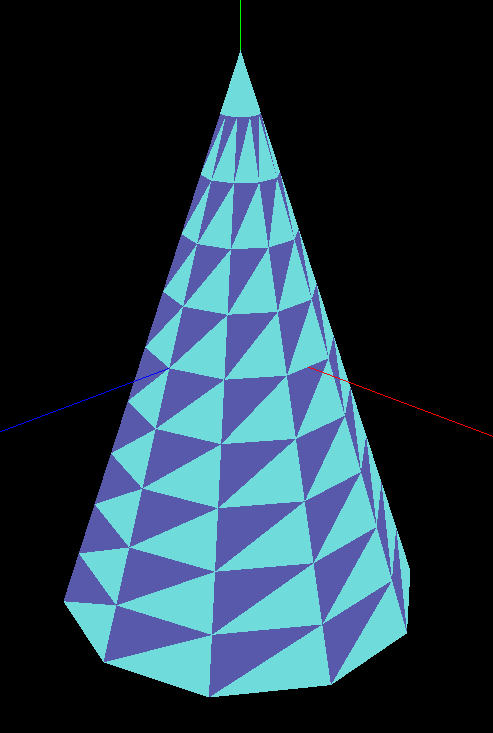
\includegraphics[width=0.7\linewidth]{images/conedraw.png}
\end{figure}

\vspace{0.5cm}

Tal como na esfera, as camadas horizontais e verticais formam entre si um retângulo que por sua vez está dividido em dois triângulos.

\subsubsection{Cálculo das coordenadas e das variações de $r'$}

Mais uma vez, o processo é um pouco semelhante com o da esfera, porque em cada camada, haverá uma circunferência que contém os pontos do cone naquela altura exata, a principal diferença aqui é o cálculo da coordenada Y porque não iremos ter nenhum vetor com tamanho igual ao raio que ligue o ponto à origem da esfera, então precisamos de utilizar a semelhança de triângulos para calcular o valor da coordenada Y.

\begin{figure}[h]
\centering
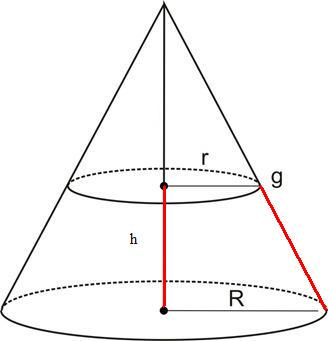
\includegraphics[width=0.5\linewidth]{images/semtri.png}
\end{figure}

\vspace{0.5cm}

Como vemos pela figura, a coordenada Y de qualquer ponto presente na circunferência representada pelo raio $r$ será a soma de $h$ com a coordenada Y do centro da base.
Sabemos também que, como fazemos a divisão por stacks, o $h$ representado na figura, a cada stack, é a altura total do cone dividida pelo número de stacks pretendido.
Então para descobrir o raio $r$, sendo $heigh$ a altura total do cone e $R$ o raio da base:
\[(heigh-\frac{heigh}{stacks}) \times R = heigh \times r\]
\[\Leftrightarrow \frac{(heigh-\frac{heigh}{stacks})}{heigh} \times R = r\]
\[\Leftrightarrow (1-\frac{1}{stacks}) \times R = r\]
\[\Leftrightarrow r = R - \frac{R}{stacks}\]

\vspace{1cm}

Assim, para cada camada onde nos encontravamos o raio da circunferência seria $R$, o raio da circunferência da próxima camada seria $r$ e seria calculado por $r = R - \frac{R}{stacks}$. 

\vspace{0.5cm}

Já tendo a coordenada Y e o raio da circunferência de cada camada, basta-nos calcular agora as restantes coordenadas.

\begin{figure}[H]
\centering
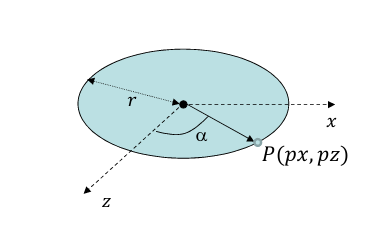
\includegraphics[width=0.6\linewidth]{images/circ.png}
\end{figure}

\[x = r \times sin (\alpha)\]
\[z= r \times cos (\alpha)\]

A diferença de alturas entre camadas será sempre $\frac{heigh}{stacks}$.

\vspace {0.5cm}

É necessário também desenhar a base, em que o pontos de todos os triângulos será sempre a origem e os restantes calculam-se a partir do ângulo $\alpha$ que cada vetor origina, vetor esse que liga qualquer ponto à origem e contém norma igual ao raio. A coordenada Y da base é constante e será na parte negativa com valor metade da altura de modo a que o cone esteja centrado na origem.

\[x = r \times sin(\alpha)\]
\[y = - \frac{heigh}{2}\]
\[z = r \times cos (\alpha)\]

\begin{figure}[H]
\centering
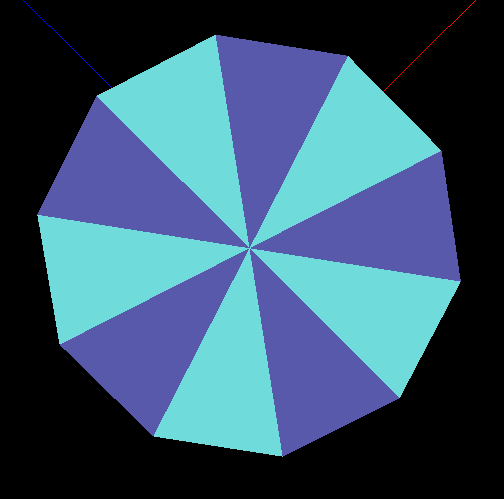
\includegraphics[width=0.5\linewidth]{images/basecone.png}
\end{figure}


\vspace{0.5cm}
\subsection{Camera}

Foi também implementado um sistema onde podemos alterar a prespetiva de visão.
Como sabemos, podemos definir a prespetiva de visão definindo um angulo $\alpha$ e $\beta$ e um $raio$ que seria a distância entre a origem e posição onde se encontra a câmara. Assim, basta alterar os valores destes parâmetros para colocar a rodar o nosso ângulo de visão sobre a origem como se andassemos à volta de uma superfície esférica. Para que seja possível utilizar estes valores, é necessário depois convertê-los para coordenadas cartesianas.

\end{document}